Graf definiuje się jako pewną parę uporządkowaną $G = (V, E)$, gdzie $V$ to~zbiór wierzchołków,
a $E$ to~zbiór krawędzi.
Takie obiekty przedstawić graficznie jako zbiór punktów (wierzchołków) rozmieszczonych w~płaszczyźnie,
połączonych łukami (krawędziami), które odpowiadają połączeniom między tymi wierzchołkami.
Każda krawędź może być interpretowana jako ciągła linia łącząca parę wierzchołków,
przy czym linie te mogą być dowolnie zakrzywione,
ale nie mogą się przecinać z~innymi w~sposób tworzący wielokrotne punkty.
Grafy można wykorzystywać do reprezentacji danych, relacji między nimi oraz modelowania złożonych struktur.
Według \cite{Wloch2008} grafy „\textit{stanowią wygodny aparat do modelowania różnych obiektów, (...) i~odpowiednio interpretowane
- mogą zawierać pewne informacje}”.

Teoria grafów to~dziedzina matematyki zajmująca się badaniem właściwości grafów,
będąca bardzo ważnym narzędziem w~wielu „\textit{dziedzinach od rachunku operacyjnego, chemii, po genetykę, lingiwistykę
oraz od elektroniki i~geografii po socjologię i~architekturę}”\cite{Wilson2012}.
Grafy dają możliwość zobrazowania pewnych modeli, co jest szczególnie korzystne w~analizie wzorców.
W kontekście grafów warto podkreślić ich zastosowanie poza teoretycznymi analizami.

W dziedzinach informatycznych, grafy stanowią fundament wielu algorytmów, takich jak algorytmy przeszukiwania,
algorytmy najkrótszej drogi, drzew rozpinających, czy modeli sieci.
Przykładem może być tutaj wyszukiwanie najkrótszej trasy, chociażby w~nawigacji GPS,
gdzie wierzchołki odpowiadają skrzyżowaniom, a~krawędzie drogom.
W przypadku znajdowania najbardziej optymalnych tras, warto wymienić takie algorytmy jak $A^*$, Bellmana-Forda czy Dijkstry.

\begin{figure}[ht]
	\centering
	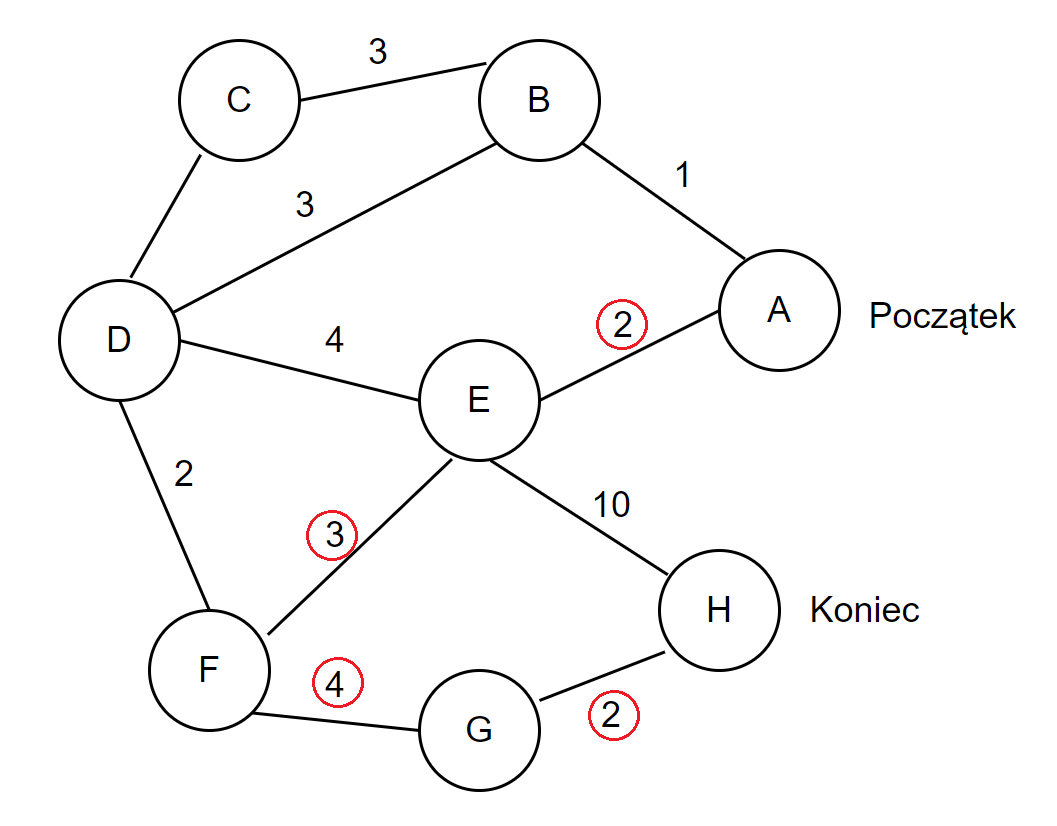
\includegraphics[height=5.6cm]{resources/introduction/images/shortest_path.png}
	\caption{Przykład grafu z~wyznaczoną najkrótszą drogą od wierzchołka $A$ do $H$.
		Zaznaczona została czeronymi okręgami.
		Liczby przy krawędziach grafu oznaczają odległość między wierzchołkami łączonymi daną krawędzią.}
    \label{Fig:intro-1}
\end{figure}
\FloatBarrier

Grafy istotną rolę odgrywają w~reprezentacji i~modelowaniu struktur danych, takich jak bazy danych.
Najczęściej stosowane bazy danych, tj. relacyjne, zbudowane są w~sposób, który grafy mogą doskonale zobrazować -
wierzchołki odpowiadają kolumnom w~tabelach a~połączenia między nimi to~krawędzie, reprezentujące relacje.

\begin{figure}[ht]
	\centering
	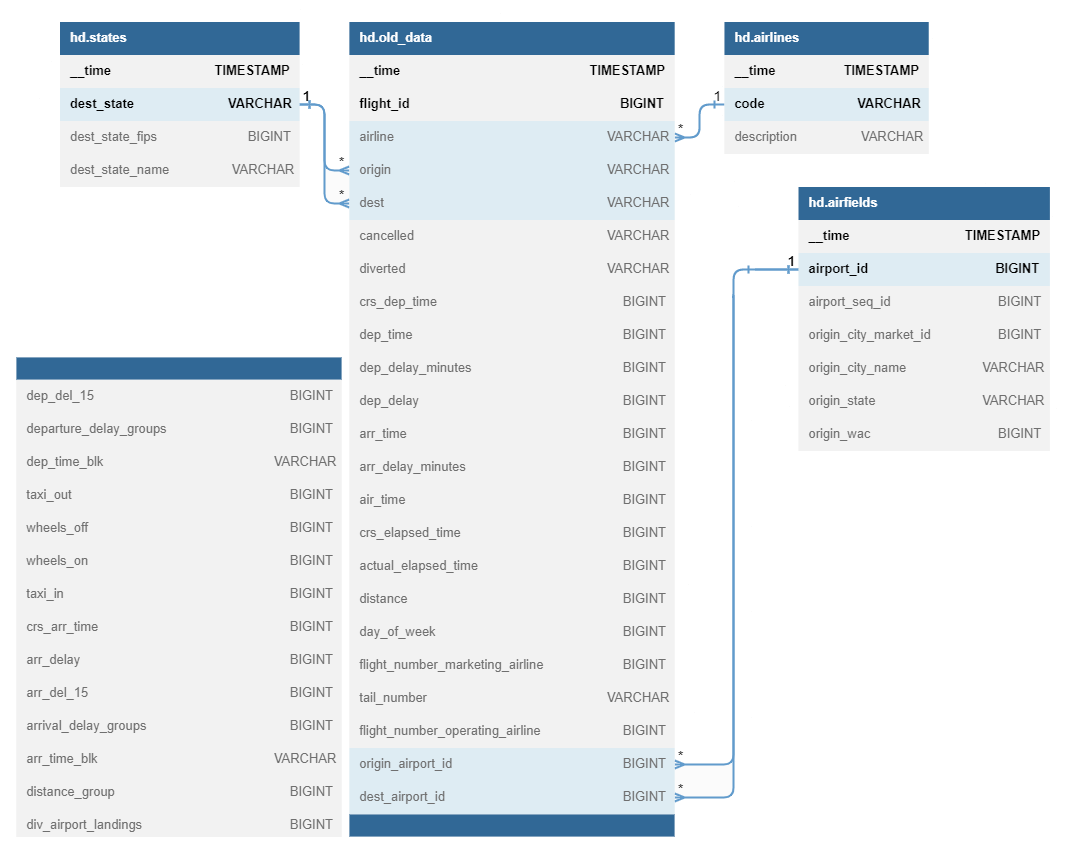
\includegraphics[height=7.5cm]{resources/introduction/images/database.png}
	\caption{Przykładowy schemat relacyjnej bazy danych.
		Źródło: opracowanie własne na~podstawie danych:
		https://www.kaggle.com/datasets/robikscube/flight-delay-dataset-20182022}
    \label{Fig:intro-2}
\end{figure}
\FloatBarrier

\clearpage

W biologii grafy pełnią ważną rolę w~modelowaniu układu nerwowego, sieci białek,
szlaków metabolicznych oraz interakcji między genami \cite{Chung2021}.
W genetyce wykorzystuje się je między innymi do analizy drzew filogenetycznych,
co pozwala chociażby na~śledzenie relacji ewolucyjnych między organizmami,
z wierzchołkami stopnia 1 reprezentującymi żywe organizmy,
a wierzchołkami pośrednimi jako ich wspólnymi przodkami \cite{Erciyes2023}.

\begin{figure}[ht]
	\centering
	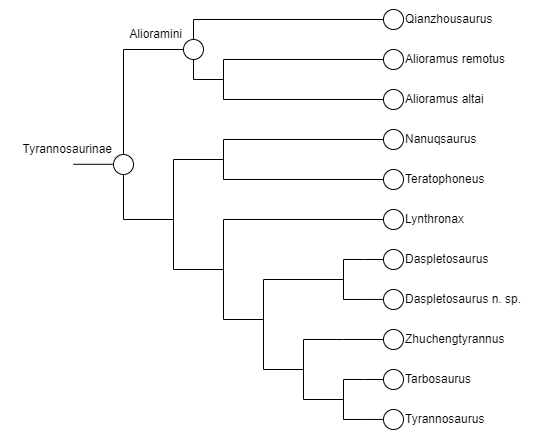
\includegraphics[width=12cm]{resources/introduction/images/dino.png}
	\caption{Filogenetyczne relacje podrodzin dinozaurów rodziny Tyrannosaurinae.
		Źródło: opracowanie własne na~podstawie:
		Brusatte, S., Carr, T.: \textit{The phylogeny and evolutionary history of tyrannosauroid dinosaurs}. Scientific Reports 6, 20252, 2016}
    \label{Fig:intro-3}
\end{figure}
\FloatBarrier

Natomiast w~chemii grafy służą do reprezentacji struktury molekularnej związków chemicznych,
umożliwiając naukowcom analizę ich właściwości i~reaktywności.
Znaczenie teorii grafów dla chemii wynika głównie z~istnienia zjawiska izomeryzmu,
które jest uzasadnione przez teorię struktury chemicznej.
Wszystkie wzory strukturalne związków o~wiązaniach kowalencyjnych są grafami,
które nazywane są grafami molekularnymi \cite{Balaban1985}.

\begin{figure}[ht]
	\centering
	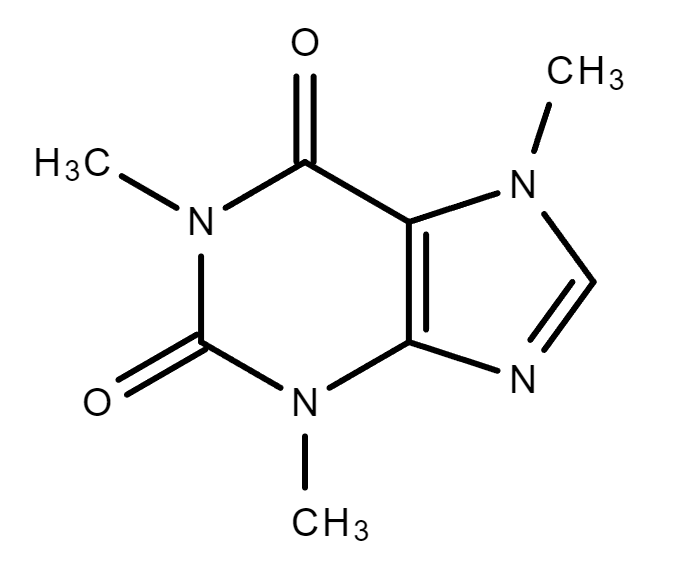
\includegraphics[height=5.5cm]{resources/introduction/images/chem.png}
	\caption{Struktura molekularna kofeiny
		Źródło: opracowanie własne na~podstawie:
		Rodak K., Kokot I., Kratz E.W.: \textit{Caffeine as a~Factor Influencing the Functioning of the Human Body-Friend or Foe?} Nutrients 13, 3088, 2021}
    \label{Fig:intro-4}
\end{figure}
\FloatBarrier

W lingwistyce, przy pomocy grafów możliwe jest modelowanie struktury języka, analiza morfologiczna czy syntaktyczna.
Stosowane są również przez wiele innych dziedzin, takich jak gramatyka generatywna,
będąca kandydatem na~teoretyczną podstawę biolingwistyki.
Przez ponad pół wieku, wykorzystywała ona notację drzewa jako pomocnicze narzędzie do wyrażania struktur językowych,
lecz takie podejście zostało ostatecznie podważone przez jednego z~autorytetów w~dziedzinie lingwistyki - Noama Chomsky'ego \cite{Arikawa2019}.
Dzięki grafom, możliwe jest również lepsze zrozumienie i~przetwarzanie języka naturalnego przez komputery,
co stanowi podstawę technologii takich jak tłumaczenie automatyczne czy rozpoznawanie mowy.

Teoria grafów znajduje także zastosowanie w~analizie sieci społecznych, gdzie pomagają w~badaniu relacji między ludźmi.
Wielu psychologów i~socjologów zajmuje się tematem struktur wynikających z~relacji między różnymi podmiotami.
Przykładami takich zależności mogą być sieci komunikacyjne między ludźmi, relacje dominacji i~uległości w~grupie,
wpływ lub~władza jednych podmiotów nad innymi, czy relacje między różnymi aspektami pola psychologicznego danej osoby lub~jej osobowości \cite{Harary1953}.
Bardzo dużym polem jest również analiza mediów społecznościowych, które to~wpływają coraz bardziej na~przeciętnego człowieka.
Poprzez gromadzenie i~analizę danych dotyczących połączeń między użytkownikami, wzorców interakcji i~zachowań komunikacyjnych,
analiza mediów społecznościowych pozwala zauważyć pewne struktury społeczne i~zidentyfikować wzorce leżące u podstaw interakcji w~ich obrębie.
Wszystko to~możliwe jest do modelowania za pomocą struktur znanych z~teorii grafów \cite{Umami2024}.

\begin{figure}[ht]
	\centering
	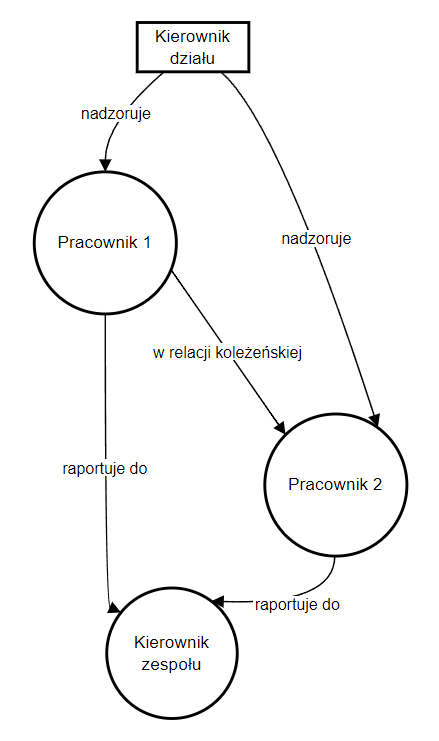
\includegraphics[height=8.5cm]{resources/introduction/images/social.png}
	\caption{Przykład sieci relacji pomiędzy pracownikami w~dziale danej firmy}
    \label{Fig:intro-5}
\end{figure}
\FloatBarrier

Rozpoznawanie wzorców, nam ludziom, pozwala na~szybszą naukę przez rozpoznawanie czegoś, co już wcześniej widzieliśmy.
W bardzo dużym uproszczeniu, algorytmy uczenia maszynowego działają w~podobny sposób.
Gdy model zostanie prawidłowo nauczony na~pewnych danych,
jest w~stanie rozpoznawać podobne wzorce w~innych, nigdy wcześniej nie widzianych.

Podsumowując, grafy są niezwykle wszechstronnym narzędziem,
które znajduje zastosowanie w~bardzo wielu dziedzinach nauki i~technologii.
Ich zdolność do reprezentowania skomplikowanych struktur i~relacji w~sposób zrozumiały, przystępny i~czytelny jest nieoceniona.
Dzięki nim możliwe jest również analizowanie i~przetwarzanie informacji w~efektywniejszy sposób,
niż informacji nieustrukturyzowanych. 

Celem pracy jest zobrazowanie owej zależności, na~przykładzie nauczenia sieci neuronowej,
w taki sposób, by po wytrenowaniu na~kilku typach grafów stworzonych sztucznie,
model był w~stanie rozpoznać dane wzorce i~je nazwać, w~przestrzeni rzeczywistej.